\section{My work and its place in the institute: description and analysis}
\label{sec:work}

\subsection{Assignment, role and working environment}
\label{sec:setup}

In the team's workflow I acted as an investigator inside an existing code base.
SMILify supplied the parametric representation and a baseline
optimisation-based fitting pipeline; I added the diagnostic and validation
machinery around it and the extensions evaluated with it
(Table~\ref{tab:contrib}). Every extension was judged against a criterion
registered before the experiment was run, so that a favourable-looking result
could not be reinterpreted afterwards.

\begin{table}[!htb]
\centering
\caption{Components of the repository I implemented or extended.}
\label{tab:contrib}
\begin{tabular}{@{}L{0.36\linewidth}L{0.56\linewidth}@{}}
\toprule
\textbf{Component} & \textbf{Contribution}\\
\midrule
Preprocessing & Implemented and extended (Alpha Wrap, ManifoldPlus, cleanup,
 quadric-error reduction)\\
Joint limits & Integrated into the 3D registration path\\
Correspondence benchmark, synthetic corpus & Implemented\\
PointNet initialisation & Integrated and evaluated\\
SDF analysis, chain-aware assignment & Implemented and evaluated\\
Evaluation harness, Joint Alignment Benchmark & Designed and implemented\\
HPC pipeline & Configured on two systems\\
Morphometric analysis & Implemented\\
\bottomrule
\end{tabular}
\end{table}

The stack is Python, PyTorch~2.3.1, PyTorch3D~0.7.8~\cite{pytorch3d}, NumPy,
SciPy, Trimesh, Blender and a CGAL-based Alpha Wrap, with YAML-configured
experiments under Git. Each fit is a non-linear optimisation over about
$10^4$ vertices, and the study comprised many ablations over many specimens and
seeds. It therefore ran on J\"ulich's JURECA (CUDA~11.8) and on an RWTH
allocation with H100 GPUs (CUDA~13.0), several thousand GPU-hours in total, as
batch jobs with recorded seeds, preserved checkpoints and intermediate fitting
stages, and a hash-frozen benchmark.

\subsection{Technical framework}
\label{sec:framework}

\subsubsection{The SMIL model and the registration objective}

The model has a fixed-topology template of $10{,}235$ vertices, a kinematic
tree of $55$ joints, per-vertex skinning weights, a $25$-dimensional shape
basis, a bilateral symmetry map and authored joint rotation limits. Fixed
topology is what makes correspondence possible: vertex $i$ denotes the same
anatomical locus in every fit, so quantities such as head width become
comparable across specimens without a further alignment step. A shaped vertex
$\bar{\mathbf v}_i(\bm\beta)=\mathbf v^{0}_i+\sum_k\beta_k\mathbf s_{ik}$ is
posed by linear blend skinning:
\begin{equation}
\mathbf v_i(\bm\beta,\bm\theta)=\sum_{j=1}^{55} w_{ij}\,G_j(\bm\theta)\,\bar{\mathbf v}_i(\bm\beta),
\qquad G_j(\bm\theta)=\prod_{k\in\mathrm{anc}(j)}\big[R(\theta_k)\,|\,\mathbf t_k\big],
\label{eq:lbs}
\end{equation}
where $w_{ij}$ are skinning weights and $G_j$ composes the transforms of all
ancestors of joint $j$. Two consequences matter later. A rotation error at a
proximal joint changes $G_j$ for every descendant and so displaces everything
distal to it. And the surface depends on joint \emph{positions} only through
$G_j$, so a surface can look right while the skeleton inside it is wrong.

Figure~\ref{fig:pipeline} shows the pipeline: preprocessing, initialisation,
registration and, new in this internship, a correspondence-audit stage that
reports how far each vertex's identity can be trusted rather than only how
close the surfaces are. Registration (Equation~\ref{eq:registration}) is
solved by gradient-based optimisation with PyTorch3D~\cite{pytorch3d},
minimising $\mathcal{L}=\sum_t\lambda_t\mathcal{L}_t$ in four stages (global
pose and scale, then posing, then coarse and fine vertex deformation).
Table~\ref{tab:objective} states what each term \emph{observes}, which is the
information the optimiser actually has.

\begin{figure}[!htb]
\centering
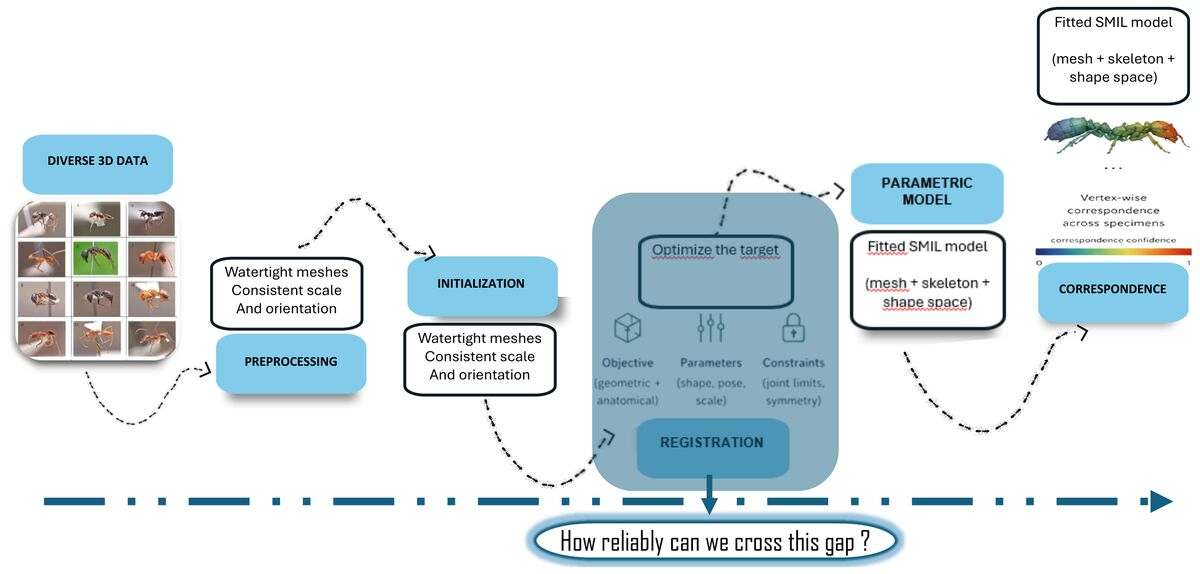
\includegraphics[width=0.82\linewidth]{figures/fig_pipeline_full.jpg}
\caption[The registration pipeline]{The registration pipeline, from diverse
raw scans to a fitted parametric model with vertex-wise correspondence. The
correspondence stage did not exist before this internship.}
\label{fig:pipeline}
\end{figure}

\begin{table}[!htb]
\centering
\caption{Terms of the registration objective and what each one observes.}
\label{tab:objective}
\begin{tabular}{@{}L{0.24\linewidth}L{0.68\linewidth}@{}}
\toprule
\textbf{Term} & \textbf{What it observes}\\
\midrule
Chamfer & Distance from sampled model points to the nearest target point and
 back; a function of two surfaces, blind to which vertex is which\\
Normal & Agreement of surface normals at matched points\\
Edge, Laplacian, offset & Mesh regularity and size of the residual
 deformation $\mathbf d$ (ARAP-style~\cite{arap}); independent of the target\\
Symmetry, midline & Bilateral consistency of the model\\
Rotation limits & Joint \emph{angles} against authored ranges, not joint
 positions\\
\bottomrule
\end{tabular}
\end{table}

No term takes a joint location or a vertex identity as an observation. The
surface term is evaluated on $N$ sampled points,
$\mathcal{L}_{\mathrm{ch}}\approx\frac1N\sum_i d(p_i,T)^2$, so the sampling
distribution is itself an implicit weighting over anatomy.

\subsubsection{Preprocessing, initialisation and related work}

Scans arrive with holes, disconnected fragments, non-manifold geometry and
thin appendages that vanish under naive simplification. Two complementary
repairs were evaluated. Alpha Wrap~\cite{alphawrap} builds a new watertight
envelope around arbitrarily damaged input; its single scale parameter trades
vanishing thin structures (too coarse) against surviving defects (too fine).
ManifoldPlus~\cite{manifoldplus} repairs the surface directly and served as a
fallback. Conservative cleanup and topology-preserving quadric-error-metric
reduction~\cite{qem} complete the stage. On 44 processed specimens, $44$ of
$44$ meshes were watertight and $29$ of $44$ were reduced to a single
connected component, a substantial improvement in topology, and the pipeline
was retained. Initialisation uses a PointNet-style encoder~\cite{pointnet} that
predicts shape, pose and global transform directly from the target, instead of
a fixed canonical start.

The difficulties met here are recognised in the registration literature.
Deep Closest Point~\cite{dcp} learns point embeddings for closest-point
matching, PREDATOR~\cite{predator} predicts the overlap region of low-overlap
pairs, and GeoTransformer~\cite{geotransformer} combines geometric attention
with coarse-to-fine matching. Functional maps~\cite{fmaps} and optimal
transport~\cite{ot} offer globally consistent correspondence formulations.
This report studies a harder, model-based variant: registration constrained to
the image of an articulated parametric model, where nearest-surface matching is
the local mechanism and the open question is what information it lacks.

\subsection{Methodology}
\label{sec:method}

Every result rests on one of three kinds of ground truth.

\textbf{Synthetic ground truth.} Real scans have no known vertex identities,
but the model can generate its own targets: sample $(\bm\beta,\bm\theta)$,
pose the template, optionally corrupt the mesh (noise, holes, dropped points),
strip the identities, refit with the production fitter, and compare fitted
vertex $i$ with true vertex $i$. The corpus holds $5000$ specifications drawn
with a fixed seed, pose scale $0.50$ and shape scale $2.0$, with fixed
train/test splits, so that initialisation, sampling and correspondence can be
varied one at a time. The limitation is intrinsic: the target comes from the
model, so the benchmark bounds error on real scans from below.

\textbf{Expert ground truth.} For real specimens, an expert placed 3D joints
manually. The resulting Joint Alignment Benchmark (JAB) contains eleven
annotated specimens and $396$ fits under a fixed protocol. Annotations were
re-registered through each mesh to a residual below $7\times10^{-8}$ and the
benchmark was frozen and hash-verified (SHA-256). Skeleton error is reported as
a percentage of Weber's length (WL), the length of the mesosoma, used as a
size-invariant unit.

\textbf{Evaluation protocol.} Surface proximity can be gamed. A direct
adversarial test, snapping distal vertices onto the nearest target surface,
improves a per-part distance metric by $53\%$ while edge-length distortion
rises $7.5$-fold. The protocol therefore always combines three levels
(Table~\ref{tab:levels}), and an intervention is adopted only if it does not
degrade levels 1--2 and is checked at level 3 wherever ground truth exists.
Paired comparisons use bootstrap confidence intervals and sign or Friedman
tests; variance is attributed to joint, specimen and seed on the log scale; and
leave-one-region-out evaluation withholds supervision for one region at a time
to test whether it propagates.

\begin{table}[!htb]
\centering
\caption{The three evidence levels of the evaluation protocol, always used
together.}
\label{tab:levels}
\begin{tabular}{@{}L{0.22\linewidth}L{0.40\linewidth}L{0.30\linewidth}@{}}
\toprule
\textbf{Level} & \textbf{Metrics} & \textbf{Question answered}\\
\midrule
1. Surface proximity & Chamfer, F-score, Hausdorff, per-part variants & Does
 the mesh cover the target?\\
2. Integrity & Edge-length distortion, Laplacian and ARAP deviation, normal
 consistency & Was coverage bought by damaging the mesh?\\
3. Anatomical truth & Synthetic vertex-identity error; expert joint error &
 Is vertex $i$ on the locus it represents?\\
\bottomrule
\end{tabular}
\end{table}

\subsection{Diagnosis of the registration bottleneck}
\label{sec:diagnosis}

A single failed registration can originate at any of six points of the
pipeline, and diagnosing it requires a different question at each one
(Figure~\ref{fig:one-bad-fit}): what evidence is available in the scan; which
anatomical structure a region of the template represents; what pose the model
assumes; which target point a vertex should correspond to; whether the model
has enough freedom to hide a wrong correspondence behind a plausible surface;
and whether the optimiser can reach the best-scoring solution at all. The
following subsections answer these in turn, using the synthetic instrument of
Section~\ref{sec:method} as the common measuring stick.

\begin{figure}[!htb]
\centering
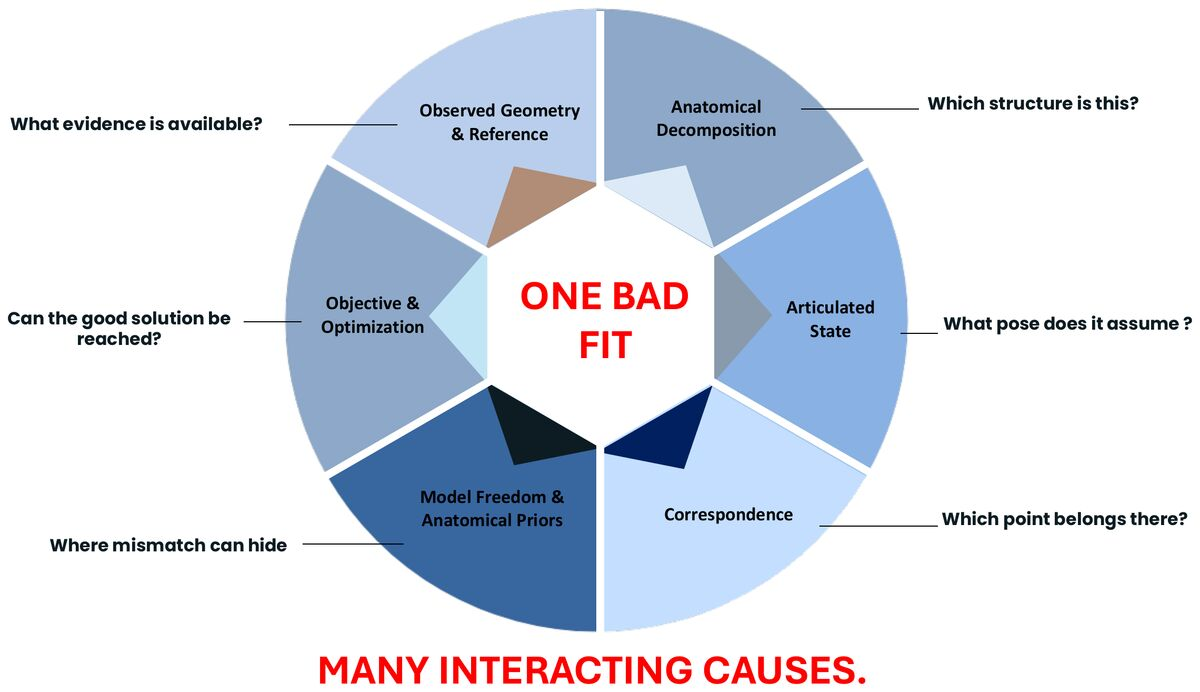
\includegraphics[width=0.5\linewidth]{figures/fig_one_bad_fit_wheel.jpg}
\caption[Six candidate causes of one bad fit]{A bad fit is rarely attributable
to a single cause: the six axes investigated here interact, and an
intervention aimed at one can leave the anatomical failure untouched.}
\label{fig:one-bad-fit}
\end{figure}

\subsubsection{Input quality is not the bottleneck (RQ1)}
\label{sec:prep-null}

Holding the registration stage fixed, the rebuilt preprocessing pipeline was
compared with the existing one by mean Chamfer distance on a matched specimen
set: $0.000771$ (new) against $0.000737$ (existing), under five percent apart
and nominally favouring the existing pipeline, although topology had improved
substantially. Mesh conditioning alone therefore does not explain the
correspondence failures (\F{F2}). Chamfer is used here only as a coverage check,
not as a test of anatomical correctness. This null result redirected the
internship from \emph{how clean is the input} to \emph{what determines whether
the optimiser finds the right correspondence at all}.

\subsubsection{Surface agreement is not anatomical correctness (RQ2)}
\label{sec:geometric-agreement}

Toggling the anatomical constraints of the objective on the same specimen set
gives the result of Figure~\ref{fig:geometric-agreement}: removing them yields
$0.45\times$ the Chamfer distance (a closer surface) but $1.25\times$ the joint
error (a worse skeleton). The fit that scores better on the objective's own
terms is the anatomically worse one (\F{F1}). The mechanism is simple once
stated: every term is a function of the two surfaces, none of which knows which
template point should represent which target point. This is the direct
motivation for the three-level protocol of Table~\ref{tab:levels}.

\begin{figure}[!htb]
\centering
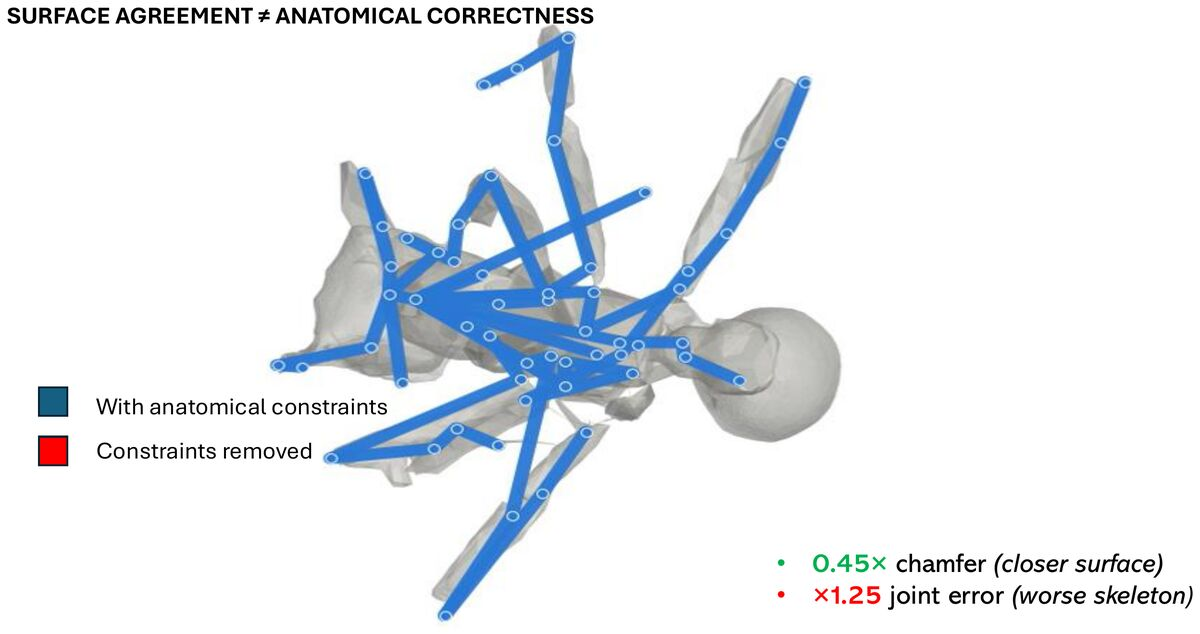
\includegraphics[width=0.6\linewidth]{figures/fig_geometric_agreement.jpg}
\caption[Surface agreement versus anatomical correctness]{Removing anatomical
constraints moves surface distance and skeleton accuracy in opposite
directions. Skeleton overlay in blue: anatomical constraints active.}
\label{fig:geometric-agreement}
\end{figure}

\subsubsection{Initialisation and articulation (RQ3)}
\label{sec:articulation}

Starting from the ground-truth pose instead of the default recovers most of the
lost accuracy for the distal chain: pretarsus error falls twelvefold
($0.1717\to0.0140$), tibia eightfold, and tarsus and femur improve
significantly ($p<0.002$). The coxa is the exception: ground-truth
initialisation is indistinguishable from a default start ($0.4204$ vs.\
$0.4114$, $p=0.47$), and the optimiser walks the coxa \emph{away} from the
correct pose it is handed, by a mean of $0.222$\,rad (\F{F4}). A matched sweep
that holds the total pose error fixed and varies only where along the chain it
sits shows why (Figure~\ref{fig:articulation-bars}): proximal error degrades
leg accuracy to $0.768$, the identical distal error only to $0.939$, because a
proximal mistake propagates through every joint downstream.

\begin{figure}[!htb]
\centering
\begin{minipage}[b]{0.46\linewidth}
\centering
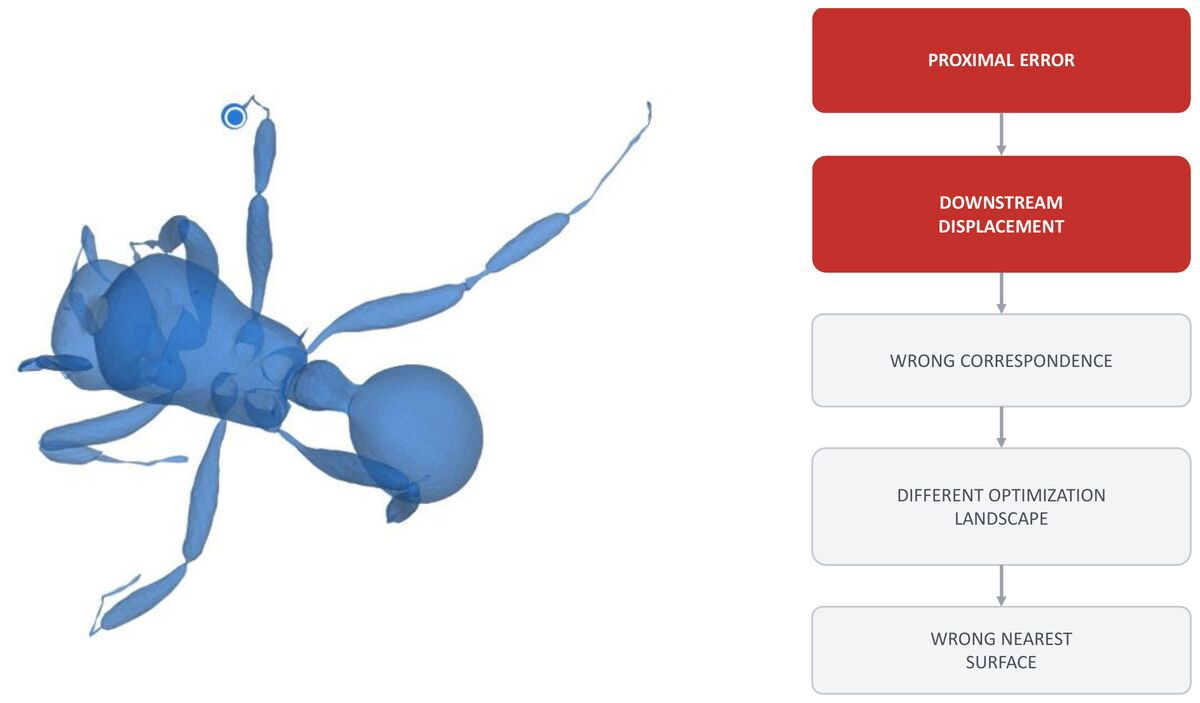
\includegraphics[width=\linewidth]{figures/fig_articulation_flow.jpg}
\end{minipage}\hfill
\begin{minipage}[b]{0.50\linewidth}
\centering
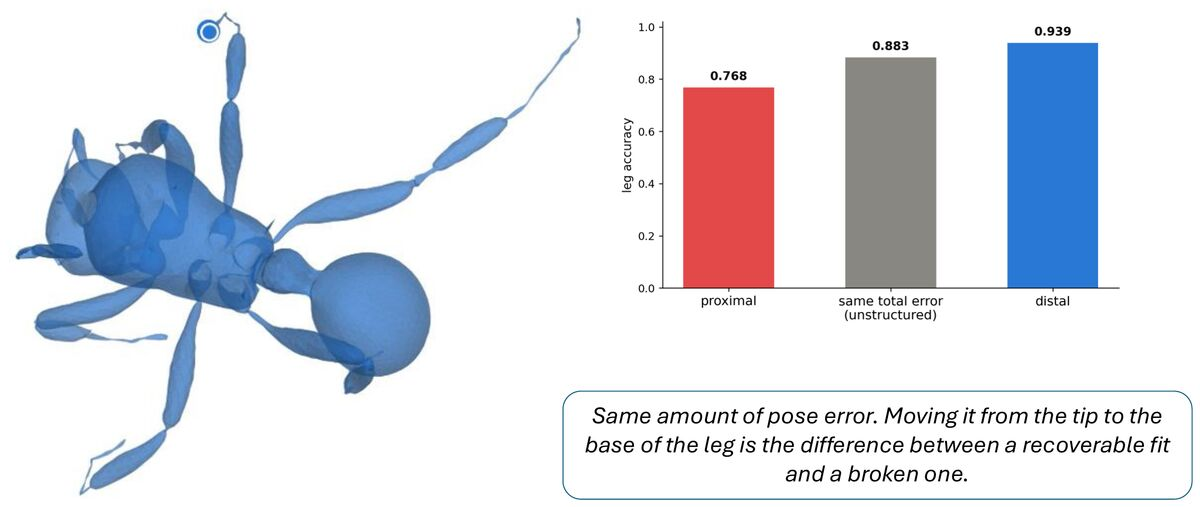
\includegraphics[width=\linewidth]{figures/fig_articulation_bars.jpg}
\end{minipage}
\caption[Pose error along the kinematic chain]{Left: a pose error near the
body propagates to everything distal to it. Right: leg accuracy for the same
total pose error placed at different points of the chain: distal $0.94$,
proximal $0.77$.}
\label{fig:articulation-bars}
\end{figure}

A learned initialiser was the natural remedy. On synthetic data it wins clearly
(leg accuracy $0.857\to0.901$, Chamfer $0.000264\to0.000226$). On 50 real
specimens, however, it is \emph{worse} than the zero-initialised default
($0.000697$ against $0.000637$ mean Chamfer, winning only 20 of 50), and
retraining at smaller perturbation magnitudes only moves it toward parity.
This is consistent with a synthetic-to-real distribution mismatch; it does not
show that the architecture cannot generalise under a more representative
training distribution. The initialiser is therefore rejected as evaluated and not deployed
(Table~\ref{tab:interventions}). The coxa result is the more consequential, since no improvement
of the initialiser can fix it.

\subsubsection{Regional identity versus localisation}
\label{sec:oracle}

An \emph{oracle intervention} supplies the fitter with the correct answer to
exactly one sub-question, and the residual error then localises the bottleneck
without proposing a deployable fix (Table~\ref{tab:oracles}). Giving every
target point its true region raises leg accuracy only from $0.867$ to $0.937$:
a large share of the error survives even when \emph{which structure is this?}
is answered perfectly, so regional identity and within-region localisation are
distinct problems (\F{F3}). A second oracle supplying near-exact per-vertex
correspondence, even at very high weight, still leaves residual error: the
other objective terms, deformation freedom and the optimisation trajectory
keep limiting the fit. Correspondence is therefore not the \emph{only} missing
ingredient; the problem lies in its interaction with objective, trajectory and
deformation.

\begin{table}[!htb]
\centering
\caption{Oracle interventions, ordered by the amount of information supplied.}
\label{tab:oracles}
\begin{tabular}{@{}L{0.20\linewidth}L{0.20\linewidth}L{0.24\linewidth}L{0.24\linewidth}@{}}
\toprule
\textbf{Oracle} & \textbf{Supplied} & \textbf{What remains} & \textbf{Evidence}\\
\midrule
Regional identity & Which structure & Error inside the correct structure &
 Leg accuracy $0.867\to0.937$\\
Dense correspondence & Where, per vertex & Objective, deformation and
 trajectory effects & Residual error persists\\
Expert joints & True skeleton & No propagation to unsupervised regions &
 $25.1\%\to17.4\%$ WL\\
\bottomrule
\end{tabular}
\end{table}

\subsubsection{Deformation freedom as an escape hatch}
\label{sec:deformation-freedom}

The objective includes free per-vertex deformation, bounded only by edge-length
and Laplacian regularisation, because the shape space cannot represent every
idiosyncrasy of a real specimen. Mechanically this is also an escape hatch: a
wrongly posed joint can be corrected either by rotating it to the right angle,
or by bending the mesh around the wrong angle until the surface term is
satisfied (Figure~\ref{fig:deformation-shortcut}). The two solutions can be
nearly indistinguishable by Chamfer while being anatomically unrelated, and
only the first preserves the correspondence needed for measurement. This is
the mechanism of \F{F1} at the level of a single joint. Neither an unbounded
nor a frozen deformation budget is correct, so deformation cost is treated as a
regularising penalty.

\begin{figure}[!htb]
\centering
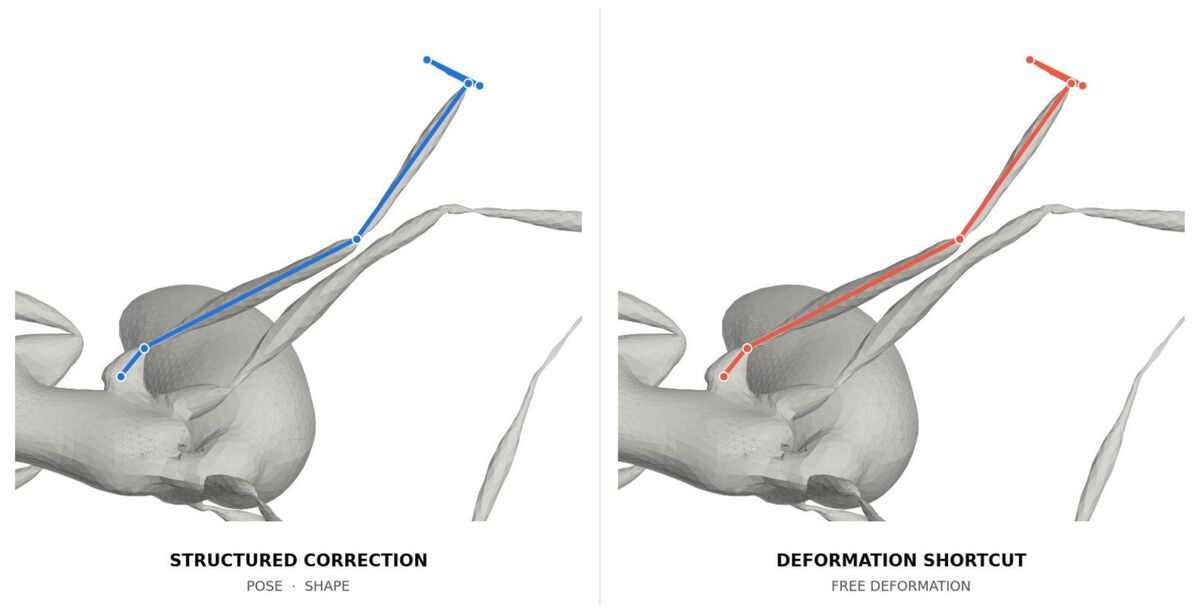
\includegraphics[width=0.58\linewidth]{figures/fig_deformation_shortcut.jpg}
\caption[Deformation as a shortcut]{Left: a structured correction through the
model's own pose and shape parameters. Right: the same visual improvement
through free per-vertex deformation, which bends the leg instead of re-posing
the joint.}
\label{fig:deformation-shortcut}
\end{figure}

\subsubsection{The objective does not constrain skeleton position}
\label{sec:skeleton-underdetermined}

Pursuing the coxa result to a mechanism first required trusting the ground
truth. An early set of expert annotations had been recorded in Blender's
internal convention, one axis permutation $(x,y,z)\mapsto(x,z,-y)$ away from
the convention of the scan meshes; every conclusion drawn against it, including
an apparent $42.7\%$ production skeleton error, was discarded (\F{F7}). On the
corrected JAB, production skeleton error is $25.1\%$ of WL (95\% CI
$17.5$--$44.8\%$). Supplying expert joint targets during fitting reduces it to
$17.4\%$ ($10$ of $11$ specimens improve). A single-factor sweep found no
existing objective term that reliably improves joint alignment (Friedman
$p=.011$, the unmodified production configuration keeping the best mean rank),
and leave-one-region-out supervision does not propagate: for every held-out
region the confidence interval of the improvement includes zero. The objective
therefore contains no explicit observation of joint location and constrains
the skeleton only indirectly (\F{F6}); this also explains why reweighting
existing terms returned null results.

The error is itself structured (Figure~\ref{fig:structured-error}). Proximal
joints are recovered far better than distal ones: coxae at $11.6\%$ of WL,
trochanter/femur at $12.9\%$, against $24$--$56\%$ for body axis, mandibles,
antennae and tibia/tarsus. A log-scale variance decomposition attributes far
more of the spread to \emph{which joint} ($0.36$) and \emph{which specimen}
($0.17$) than to the optimiser seed ($0.02$): failure is anatomically
structured, not a matter of luck (\F{F8}).

\begin{figure}[!htb]
\centering
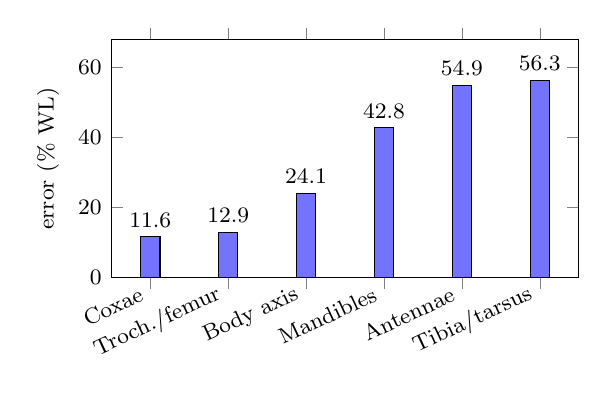
\begin{tikzpicture}
\begin{axis}[ybar,width=0.62\linewidth,height=4.6cm,bar width=7pt,ymin=0,ymax=68,
 symbolic x coords={Coxae,Troch./femur,Body axis,Mandibles,Antennae,Tibia/tarsus},
 xtick=data,x tick label style={rotate=25,anchor=east,font=\footnotesize},
 ylabel={error (\% WL)},ylabel style={font=\footnotesize},tick label style={font=\footnotesize},
 nodes near coords,every node near coord/.append style={font=\footnotesize}]
\addplot[fill=blue!55] coordinates {(Coxae,11.6)(Troch./femur,12.9)(Body axis,24.1)(Mandibles,42.8)(Antennae,54.9)(Tibia/tarsus,56.3)};
\end{axis}
\end{tikzpicture}
\hfill
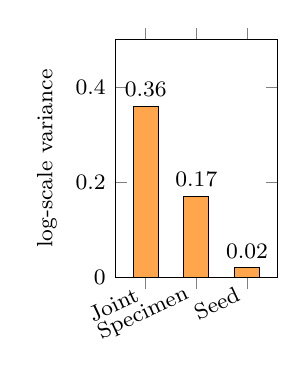
\begin{tikzpicture}
\begin{axis}[ybar,width=0.30\linewidth,height=4.6cm,bar width=9pt,ymin=0,ymax=0.5,enlarge x limits=0.3,
 symbolic x coords={Joint,Specimen,Seed},xtick=data,tick label style={font=\footnotesize},
 x tick label style={rotate=25,anchor=east},
 ylabel={log-scale variance},ylabel style={font=\footnotesize},nodes near coords,
 every node near coord/.append style={font=\footnotesize,/pgf/number format/fixed,/pgf/number format/precision=2}]
\addplot[fill=orange!70] coordinates {(Joint,0.36)(Specimen,0.17)(Seed,0.02)};
\end{axis}
\end{tikzpicture}
\caption[Structure of the skeleton error]{Left: regional skeleton error on the
corrected benchmark. Right: variance decomposition across the same fits; the
seed contributes almost nothing.}
\label{fig:structured-error}
\end{figure}

\subsubsection{Sampling, robustness and the fitting schedule}
\label{sec:sampling}

Because the surface term is a Monte Carlo estimate over $p(x)\propto$ area,
the body and head dominate and a thin distal structure is almost invisible: the
template has only $38$ tarsus and $8$ pretarsus vertices against hundreds
proximally (\F{F5}). A fixed quota for distal points helped the legs but
starved antennae and head. Starvation is a real confound, but controlling it
did not create anatomical correspondence. For points that are simply wrong,
graduated non-convexity (GNC)~\cite{gnc} treats every match as suspect at first
and hardens its confidence as optimisation proceeds. Applied to the whole body
it misbehaved around the antennae; restricted to the leg points it raised
accuracy under synthetic corruption from $0.602$ to $0.797$ (30\% of points
dropped) and from $0.411$ to $0.607$ (60\% dropped). Finally, the audit around
\F{F4} and \F{F6} exposed a defect in the staged schedule: pose was held fixed
for 2000 of the 2400 refinement iterations. Chamfer descends smoothly
regardless, so the loss curve hid it. A rebuilt schedule with a wider
pose-adjustable window improves nearly every integrity metric at no extra
cost and was shipped.

\subsection{Interventions tested}
\label{sec:interventions}

Table~\ref{tab:interventions} summarises the candidate interventions and the
outcome that the pre-registered criterion produced. Each is recorded as
hypothesis, expected mechanism, proxy metric and anatomical metric, so that a
proxy improvement cannot be mistaken for a mechanism improvement.

\begin{table}[!htb]
\centering
\caption{Candidate interventions, outcome and verdict.}
\label{tab:interventions}
\begin{tabular}{@{}L{0.30\linewidth}L{0.50\linewidth}L{0.12\linewidth}@{}}
\toprule
\textbf{Intervention} & \textbf{Outcome} & \textbf{Verdict}\\
\midrule
Joint rotation limits as a prior & Fewer impossible poses; plausible but not
 correct correspondence (\F{F1}); integrated & \verdict{ADOPT}\\
Staged schedule, pose free longer & Nearly all integrity metrics improve at no
 extra cost & \verdict{ADOPT}\\
Chain-aware anatomical assignment & Macro-F1 $0.656\to0.831$; middle-leg
 recall $0.349\to0.768$ & \verdict{ADOPT}\\
Leg-only GNC & Robustness gain under corruption (Section~\ref{sec:sampling}) &
 \verdict{HOLD}\\
Per-joint scale barrier & Outlier statistic reduced, but anterior deformation
 ratios did not move toward expected values; kept as numerical stabiliser &
 \verdict{HOLD}\\
Learned PointNet initialiser & Wins on synthetic, loses on 50 real specimens &
 \verdict{REJECT}\\
SDF instance separation & Class-level signal reliable (AUC $0.973$); one leg
 or mandible from its neighbour fails (2 of 12 specimens) & \verdict{REJECT}\\
Reweighting existing terms; anterior/posterior split & No term observes joint
 location (\F{F6}); null results & \verdict{REJECT}\\
Gaussian shape prior & Suppressed genuine shape variation; removed &
 \verdict{REJECT}\\
Probe with an untrained auxiliary network & Apparent failure traced to
 pretrained weights silently not loading & \verdict{REJECT}\\
\bottomrule
\end{tabular}
\end{table}

The Shape Diameter Function~\cite{sdf} illustrates why a descriptor can be
useful and insufficient at once. It reproduces across real scans
($r\approx0.77$--$0.94$, under $1.3$\,s per specimen) and separates body from
appendage with balanced accuracy $\approx95.1\%$. But laterality is not encoded
in local thickness: the two mandibles merged into one connected component in
$9$ of $12$ specimens, and connected components cannot separate structures that
are physically fused in the scan. Likewise, joint limits and bilateral symmetry
improve plausibility but not correspondence.

\textbf{Learned correspondence.} Four increasingly demanding tests asked
whether a learned descriptor could beat geometric matching. Normalising points
within their anatomical part performed \emph{worse} than raw coordinates, and a
first off-the-shelf learned descriptor failed at deployment through a mismatch
in point density. A within-part training objective then reduced coxa
correspondence error from $0.2689$ to $0.2247$, a $16.4\%$ improvement
(bootstrap 95\% CI $[12.6\%,19.8\%]$, $p=7.8\times10^{-26}$), so a local
descriptor does carry information raw geometry does not. Deployed as a dense,
whole-mesh field across 48 specimens, however, it is \emph{worse}: candidate-set
differences explain only $\approx2.9\%$ of a gap of roughly $145\%$, and coxa
surface coverage collapses from $28.1\%$ to $1.8\%$
(Figure~\ref{fig:local-vs-global}). The votes collapse onto a few points
instead of forming a globally consistent field. Pairwise retrieval at one joint
is not dense correspondence over a specimen, and the two must be evaluated
separately. Extrinsic learned features and a context-trained descriptor, which
beat rigid nearest-surface matching at the coxa, are the one candidate family
not bounded by the localisation ceiling of \F{F3}, and the most promising
direction.

\begin{figure}[!htb]
\centering
\begin{tikzpicture}[every node/.style={font=\small},
 n/.style={draw,rounded corners=2pt,minimum height=6.5mm,align=center,fill=white,inner sep=3pt,text width=5.6cm}]
\node[n,fill=green!12] (a) {\textbf{Local test}};
\node[n,below=2mm of a] (a2) {within-part descriptor, better pairwise retrieval};
\node[n,below=2mm of a2,fill=green!12] (a4) {$+16.4\%$ error reduction at the coxa};
\node[n,right=10mm of a,fill=red!10] (b) {\textbf{Deployment}};
\node[n,below=2mm of b] (b2) {dense correspondence field, votes collapse};
\node[n,below=2mm of b2,fill=red!10] (b4) {coverage $28.1\%\to1.8\%$};
\end{tikzpicture}
\caption[Local success versus global consistency]{The same descriptor at two
levels: strong local retrieval does not imply a usable dense correspondence
field.}
\label{fig:local-vs-global}
\end{figure}

A principle recurs across all of these results: for each intervention two
questions are asked separately, \emph{did it change its intended proxy?} and
\emph{did the anatomical mechanism the proxy stands for improve?} The
investigation repeatedly found proxy$\uparrow\not\Rightarrow$mechanism$\uparrow$:
lower Chamfer with a worse skeleton, a scale statistic that improved without
the anterior morphology improving, and a validation instrument whose own
synthetic estimate did not survive expert ground truth
(Section~\ref{sec:reliability}).

\subsection{From registration to measurement (RQ4)}
\label{sec:measurement}

The synthetic instrument shows whether the pipeline can recover a
correspondence it generated itself; it cannot show that the pipeline is right
about a real specimen. Manual 3D joint annotation by an expert provides an
independent reference (Figure~\ref{fig:ground-truth}). Against it, the
delivered fits are close to unbiased in every anatomical block, but do not
reliably \emph{rank} specimens against one another, and reliability is
structured along the body (Figure~\ref{fig:landmarks}).

\begin{figure}[!htb]
\centering
\begin{minipage}[b]{0.50\linewidth}
\centering
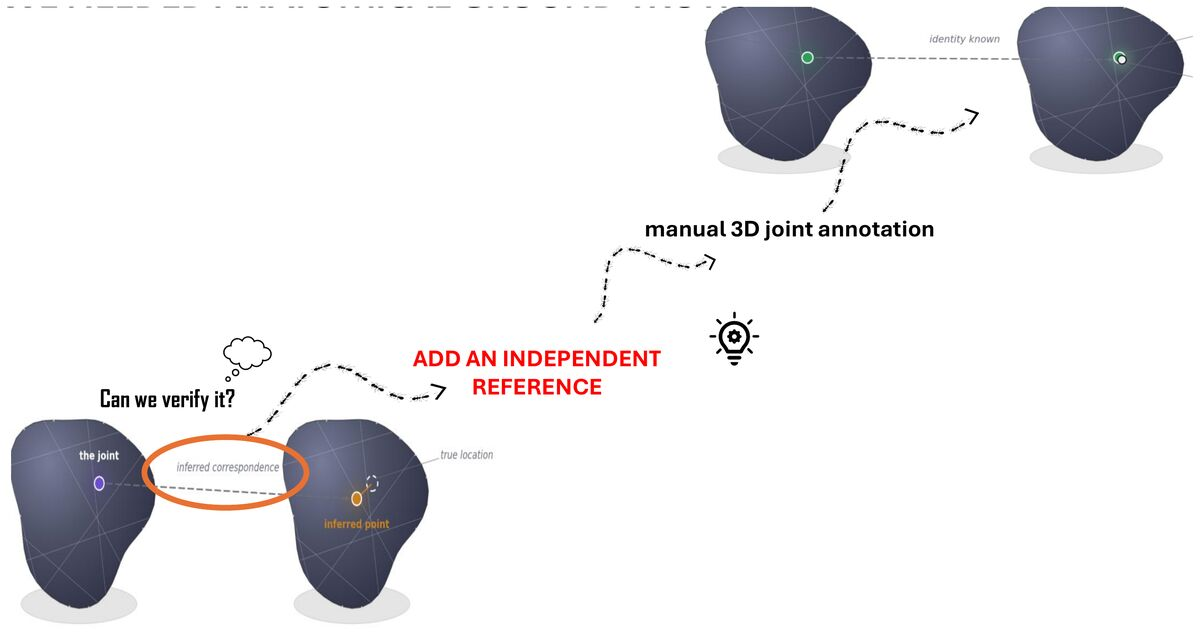
\includegraphics[width=\linewidth]{figures/fig_ground_truth_annotation.jpg}
\end{minipage}\hfill
\begin{minipage}[b]{0.38\linewidth}
\centering
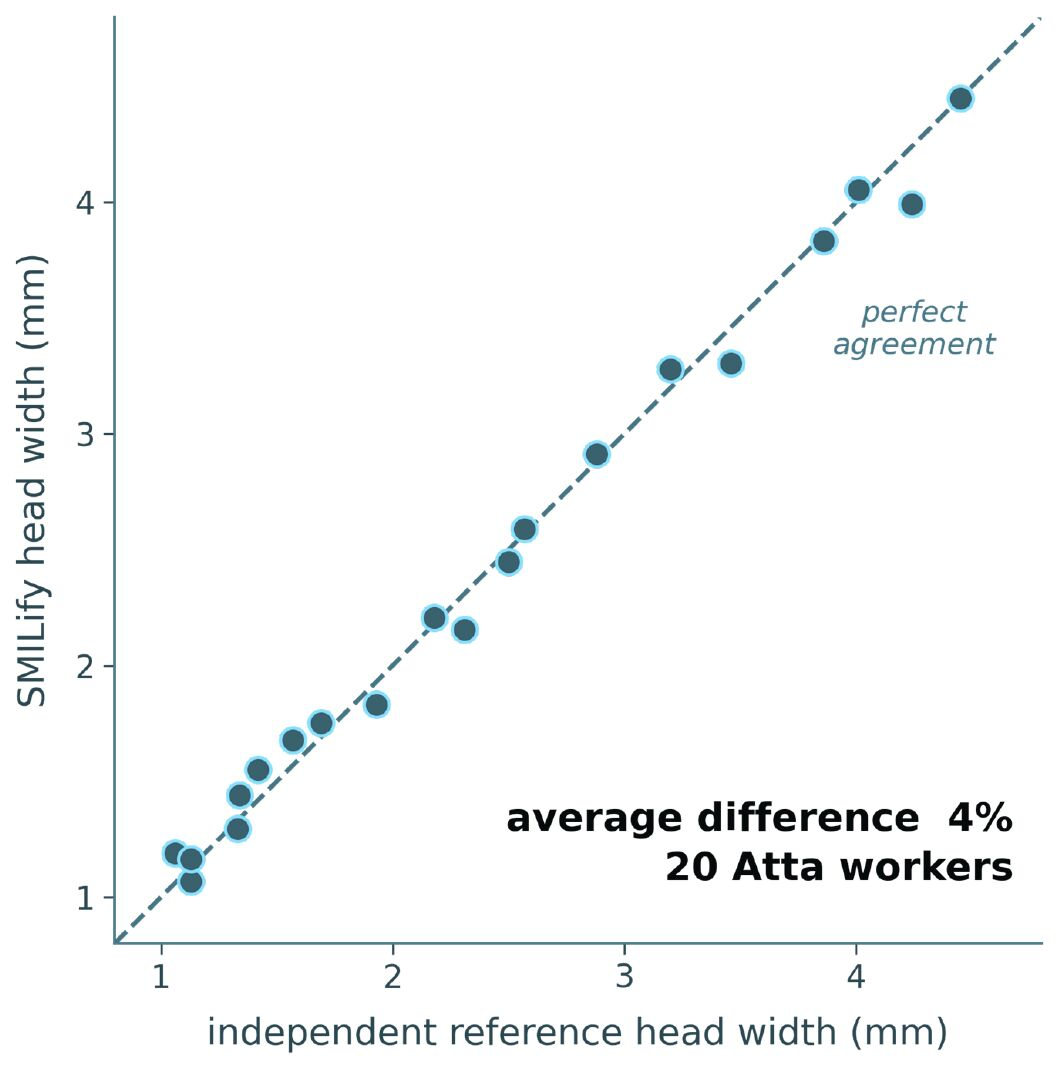
\includegraphics[width=\linewidth]{figures/fig_parameter_measurement.jpg}
\end{minipage}
\caption[Independent references]{Left: manual 3D joint annotation as an
independent reference, with identity known by construction. Right: head width
read from 20 fitted \emph{Atta} workers against an independent physical
measurement.}
\label{fig:ground-truth}
\end{figure}

\begin{figure}[!htb]
\centering
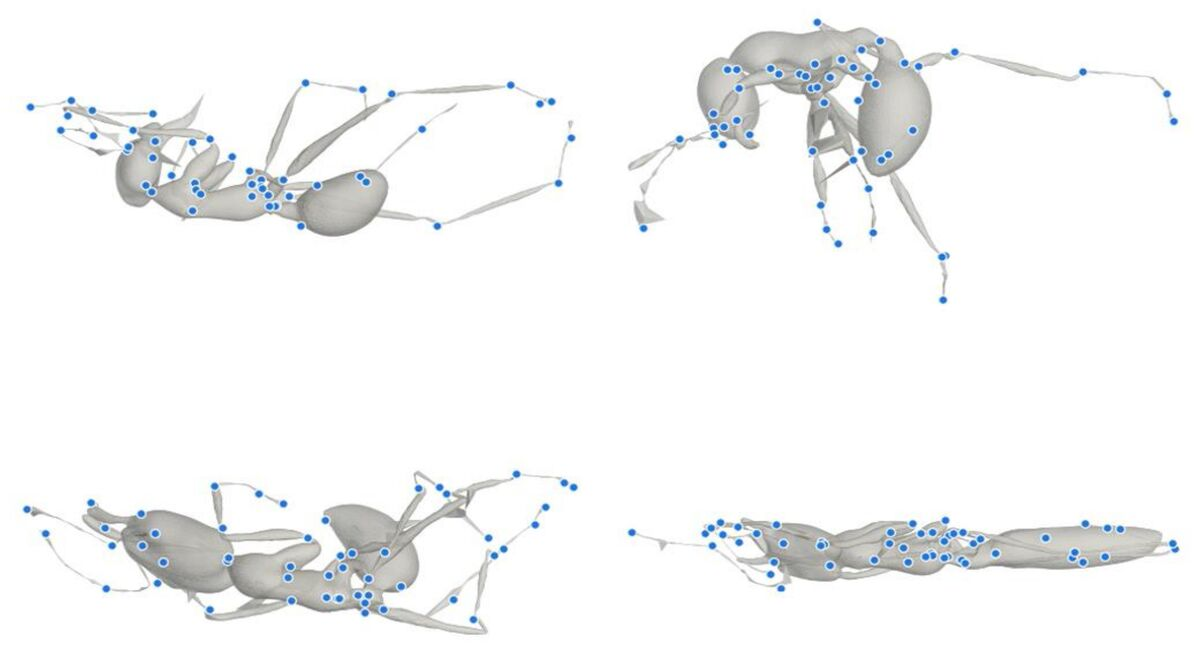
\includegraphics[width=0.58\linewidth]{figures/fig_landmarks_structured.jpg}
\caption[Structure of annotation reliability]{Expert-annotated joints across
four specimens. Reliability is not uniform: it is concentrated proximally and
degrades toward the distal leg and antenna segments, consistent with the
sampling deficit of \F{F5}.}
\label{fig:landmarks}
\end{figure}

\textbf{When a parameter becomes a measurement.} On a 20-specimen \emph{Atta}
worker corpus, joint positions recovered from the fitted model reach a median
error of $1.05\%$ of WL against expert measurements, with $96\%$ of joints
within $5\%$. Two allometric relationships (head width against body length, and
against body mass) reproduce published slopes closely ($1.189$ vs.\ $1.235$ and
$0.380$ vs.\ $0.395$) with $R^2$ between $0.987$ and $0.993$, and
Figure~\ref{fig:ground-truth} (right) shows a mean difference of $4\%$ in head width
against the physical reference. The joint-derived head-width definition showed a
smaller bias ($-0.13\%$) than a purely geometric one ($+2.22\%$) and is used
throughout. Since raw agreement in millimetres can be inherited from shared
whole-body scaling, a dimensionless ratio such as head width over body length
is the more informative target.

\textbf{Reliability of individual traits.}
\label{sec:reliability}
Against expert-corrected annotations, only one of $49$ joint-derived features
reaches a correlation of $0.5$ with ground truth. On an independent
ethanol-preserved worker corpus, registration sits at a noise floor at which
nest-mates are only $7\%$ closer than unrelated specimens, and the failing
traits are the distal leg and antenna segment lengths that \F{F5} identified as
under-sampled. Surface landmarks carry more genus-level signal than rig-derived
distances, since a rig joint is a rotation pivot rather than an anatomically
defined point; the measurement layer therefore reports surface-derived traits.
A lot-blind nearest-neighbour genus classification, tested against a permutation
null, had given encouraging results on an earlier corpus, but it could not be
re-executed in the final environment and the only available re-check (22
specimens, 9 genera) was underpowered; it is reported as provisional and is
excluded from the headline claims. Population-level aggregates are supported by
the current fits, per-specimen comparisons from joint-derived measurements are
not.

\textbf{Validity is scale-dependent.} ``The registration is valid'' is not one
claim but four, holding at different scales (Table~\ref{tab:validity}). A model
can give accurate population-level and head-width measurements while failing
to preserve the individual-level correspondence needed for specimen-by-specimen
comparison of distal segments; each statement is supported only at its own
level. The expert-supervised fit is the one result that moves skeleton accuracy
against human ground truth ($25.1\%\to17.4\%$ WL); it is demonstrated headroom
rather than a deployed capability, because expert joints are unavailable at
inference time. Supplying an equivalent signal automatically, from a learned 3D
joint predictor, is the concrete objective it motivates.

\begin{table}[!htb]
\centering
\caption{Four levels of registration validity and the evidence for each.}
\label{tab:validity}
\begin{tabular}{@{}L{0.20\linewidth}L{0.34\linewidth}L{0.34\linewidth}@{}}
\toprule
\textbf{Level} & \textbf{Question} & \textbf{Evidence}\\
\midrule
Surface correspondence & Are the surfaces close? & Chamfer, F-score
 (misleading alone, \F{F1})\\
Anatomical correspondence & Does vertex $i$ mark the same structure across
 specimens? & Synthetic oracle, expert benchmark (\F{F3}, \F{F6})\\
Parametric correspondence & Do $\bm\beta,\bm\theta$ mean the same thing across
 specimens? & Partial: 1 of 49 features reaches $r=0.5$\\
Measurement validity & Does a derived measurement match an independent one? &
 \emph{Atta} head width, allometric slopes\\
\bottomrule
\end{tabular}
\end{table}

\subsection{Summary of findings and evidence status}
\label{sec:ledger}

The results that recur are registered once and cited by identifier
(Table~\ref{tab:findings}). Beyond them, the following claims are qualified or
excluded: the scale barrier is qualified (proxy validated, mechanism
unresolved), no corpus-scale validation of it is claimed, the genus-level
permutation-null result is provisional, and functional maps, optimal transport
and canonical fields are future work.

\begin{table}[!htb]
\centering
\caption{Findings ledger: the eight load-bearing results and their evidence
status.}
\label{tab:findings}
\printfindingledger
\end{table}
